\documentclass[9pt]{report}

\usepackage{talks}
\newcommand{\expect}[1]{\mathbb{E}\!\left[ #1 \right]}
\newcommand{\reals}{\mathbb{R}}
\newcommand{\draw}[2]{#1^{(#2)}}
\usepackage{mathpazo}
\usepackage{sourcecodepro}
\usepackage{tikz}
    \usetikzlibrary{positioning, shapes, arrows.meta}

\begin{document}

\sf \mbox{}
\\[12pt]
\spc{{\LARGE\bfseries \color{MidnightBlue}{Language models for statisticians:}}
\\[4pt]
\spc{\Large\bfseries \color{MidnightBlue}{from \textit{n}-grams to
    transformers to chatbots}}
\\[24pt]
\noindent 
\spc{\large\bfseries \color{MidnightBlue}{Bob Carpenter}}
\\[2pt]
\spc{\small Center for Computational Mathematics}
\\[-1pt]
\spc{\small Flatiron Institute}
\vfill 
\noindent 
\spc{\footnotesize July 2023}
\hfill

\includegraphics[width=1.25in]{img/flatiron_logo.png}

\sld{What is a language model?}
\begin{itemize}
\item \myemph{Language} uses a \myemph{finite} number of
  symbols called \myemph{tokens}
  \subit{we assume a finite \myemph{token set} $\mathsf{Tok}$ of size $K$}
\item Tokens may be letters, words,
  sounds, syllables, etc.
  \begin{subitemize}
  \item GPT uses \myemph{sequences of letters} (average 1.5 tokens per
    English word)
  \end{subitemize}
\item Treat language as a \myemph{stochastic process}
  \subit{$Y = Y_1, Y_2, \ldots$ for random variables $Y_n \in \textsf{Tok}$}
\item Models typically \myemph{autoregressive}, predicting next
  word from previous
\end{itemize}

\sld{\textit{N}-gram language models \hfill \normalsize{(Shannon 1948)}}
\begin{itemize}
\item Assume language process is \myemph{order-\textit{N} Markov}
  \begin{subitemize}
  \item tokens conditionally independent given previous $N - 1$ tokens
    $$
    p(y_k \mid y_{k-1}, \ldots, y_1)
    = p(y_k \mid \underbrace{y_{k - 1}, \ldots, y_{k - N - 1}}_{N - 1
      \textrm{ tokens}}).
    $$
  \end{subitemize}
\item Even \myemph{GPT is Markovian}
  \begin{subitemize}
    \item GPT-3: $N = 4096$ \qquad GPT-4: $N = 8192$ \qquad Claude: $N = 100,000$
    \item \myemph{bottleneck} is $\mathcal{O}(N^2)$ attention
      algorithm (Claude more clever?)
    \item cf. a real computer is technically a finite-state machine
    \end{subitemize}
\end{itemize}
    
\sld{Shannon's \textit{N}-gram models}
\begin{itemize}
\item \myemph{Claude Shannon}. 1948. \myemph{A Mathematical Theory of Communication.}
  \textit{Bell System Technical Journal}.
\item Shannon used English \myemph{letters} ($K = 1, 2, 3$) and
  \myemph{words} ($K = 1, 2$)
\item \myemph{What is English?}  How do we collect a \myemph{sample}?
\item Shannon used \myemph{books of frequencies}
  \begin{subitemize}
  \item \myemph{letter trigrams} (1939 book); \myemph{word bigrams} (1923 book)
  \end{subitemize}
\item Fit and inference usually \myemph{regularized MLE} for efficiency
  \begin{subitemize}
  \item ensures \myemph{non-zero probability} for any sequence
  \end{subitemize}
  
\end{itemize}

\sld{Shannon's fit}
\begin{itemize}
\item MLE probabilities from compiled tables of letters (1923), words 
      (1939) 
    \subit{or, open books at random, find current context, generate 
        following word}
\item Shannon generated random examples
  \begin{subitemize}
    \item \footnotesize \myemph{Order 1, letters}: OCRO HLI RGWR NMIELWIS EU LL NBNESEBYA TH EEI ALHENHTTPA OOBTTVA
      NAH BRL.
    \item \footnotesize \myemph{Order 3, letters}: IN NO IST LAT WHEY CRATICT FROURE
      BIRS GROCID PONDENOME OF DEMONSTURES OF THE REPTAGIN IS
      REGOACTIONA
      % CRE.
    \item \footnotesize \myemph{Order 1, words}: REPRESENTING AND SPEEDILY IS AN
      GOOD APT OR COME CAN DIFFERENT NATURAL HERE HE THE A IN CAME THE
      TO
      % GRAY COME TO FURNISHES THE LINE MESSAGE HAD BE THESE.
      \item \footnotesize \myemph{Order 2, words}: THE HEAD AND IN FRONTAL ATTACK ON
        AN ENGLISH WRITER THAT THE CHARACTER OF THIS POINT IS
        THEREFORE
        % METHOD FOR THE LETTERS THAT THE TIME OF WHO EVER TOLD THE PROBLEM FOR AN UNEXPECTED.
  \end{subitemize}
\end{itemize}

\sld{Measuring accuracy with entropy}
\begin{itemize}
\item Accuracy of $N$-gram language model $p_Y$ measured with
  \myemph{entropy (rate)}
\item Given a random sequence $Y \in \textsf{Tok}^K,$ its
  \myemph{entropy} in \myemph{bits} (base 2) is
  $$
  \textrm{H}[Y]
  \ = \ \mathbb{E}\!\left[ \log_2 p_Y(Y) \right]
  \ = \ \sum_{y \in \textsf{Tok}^K} p_Y(y) \cdot \log_2 p_Y(y).
  $$
\item The \myemph{entropy rate} is average entropy per token, $\lim_{K \rightarrow \infty} \,
  \textrm{H}[Y] / K,$
\item The entropy rate for $N$-grams is given by \myemph{conditional entropy},
$$
    \textrm{H}[Y_K \mid Y_{K - 1}, \ldots, Y_{K - N - 1}]
    \ = \ \mathbb{E}\!\left[\, \log_2 p(Y_K \mid Y_{K - 1}, \ldots,
        Y_{K - N - 1}) \, \right]
$$
\end{itemize}

\sld{Signal processing: entropy and compression}
\begin{itemize}
\item Shannon (1948) introduced \myemph{information theory} to model
  \myemph{signal compression} and decompression for communication
\item Assume a language model with pmf $p_Y$
\item \myemph{Compress} $y \in \textsf{Tok}^*,$ to $\lceil \log_2 p_Y(y) \rceil$ bits
\subit{in practice with \myemph{arithmetic
    coding} (Witten, Neal, Cleary 1987)}
\end{itemize}

\sld{OpenAI's GPT-3: Published}
\begin{itemize}
\item \myemph{Training set} sizes \\[8pt]
  \small
  \begin{tabular}[t]{r|r}
    \myemph{Source} & \myemph{Tokens} \\ \hline
    Common Crawl & 410 billion  \\
    Books2 & 55 billion \\
    WebText2 & 19 billion \\
    Books1 & 12 billion \\
    Wikipedia & 3 billion \\ \hline \hline
    & $\approx$ 500 billion
  \end{tabular}
\item \myemph{Number of parameters}: $\approx$175 billion
  \vfill
\item \myemph{Context history size}: 4K tokens
\item Let's turn to \myemph{how it works $\ldots$}
\end{itemize}

\sld{Top-level architecture}
\begin{itemize}
\item \myemph{Transformer}, but \myemph{decoder only}
\item $\textsf{tok}_n$:  $n$-th \myemph{input token}
\item $x^k_n$: \myemph{value of token} $n$ at layer $k$
\item $\textsf{prob}_t$: \myemph{probability next token} is $t$
\item \myemph{circles} enclose model parameters
\end{itemize}
\vspace*{-1.75in}
\hfill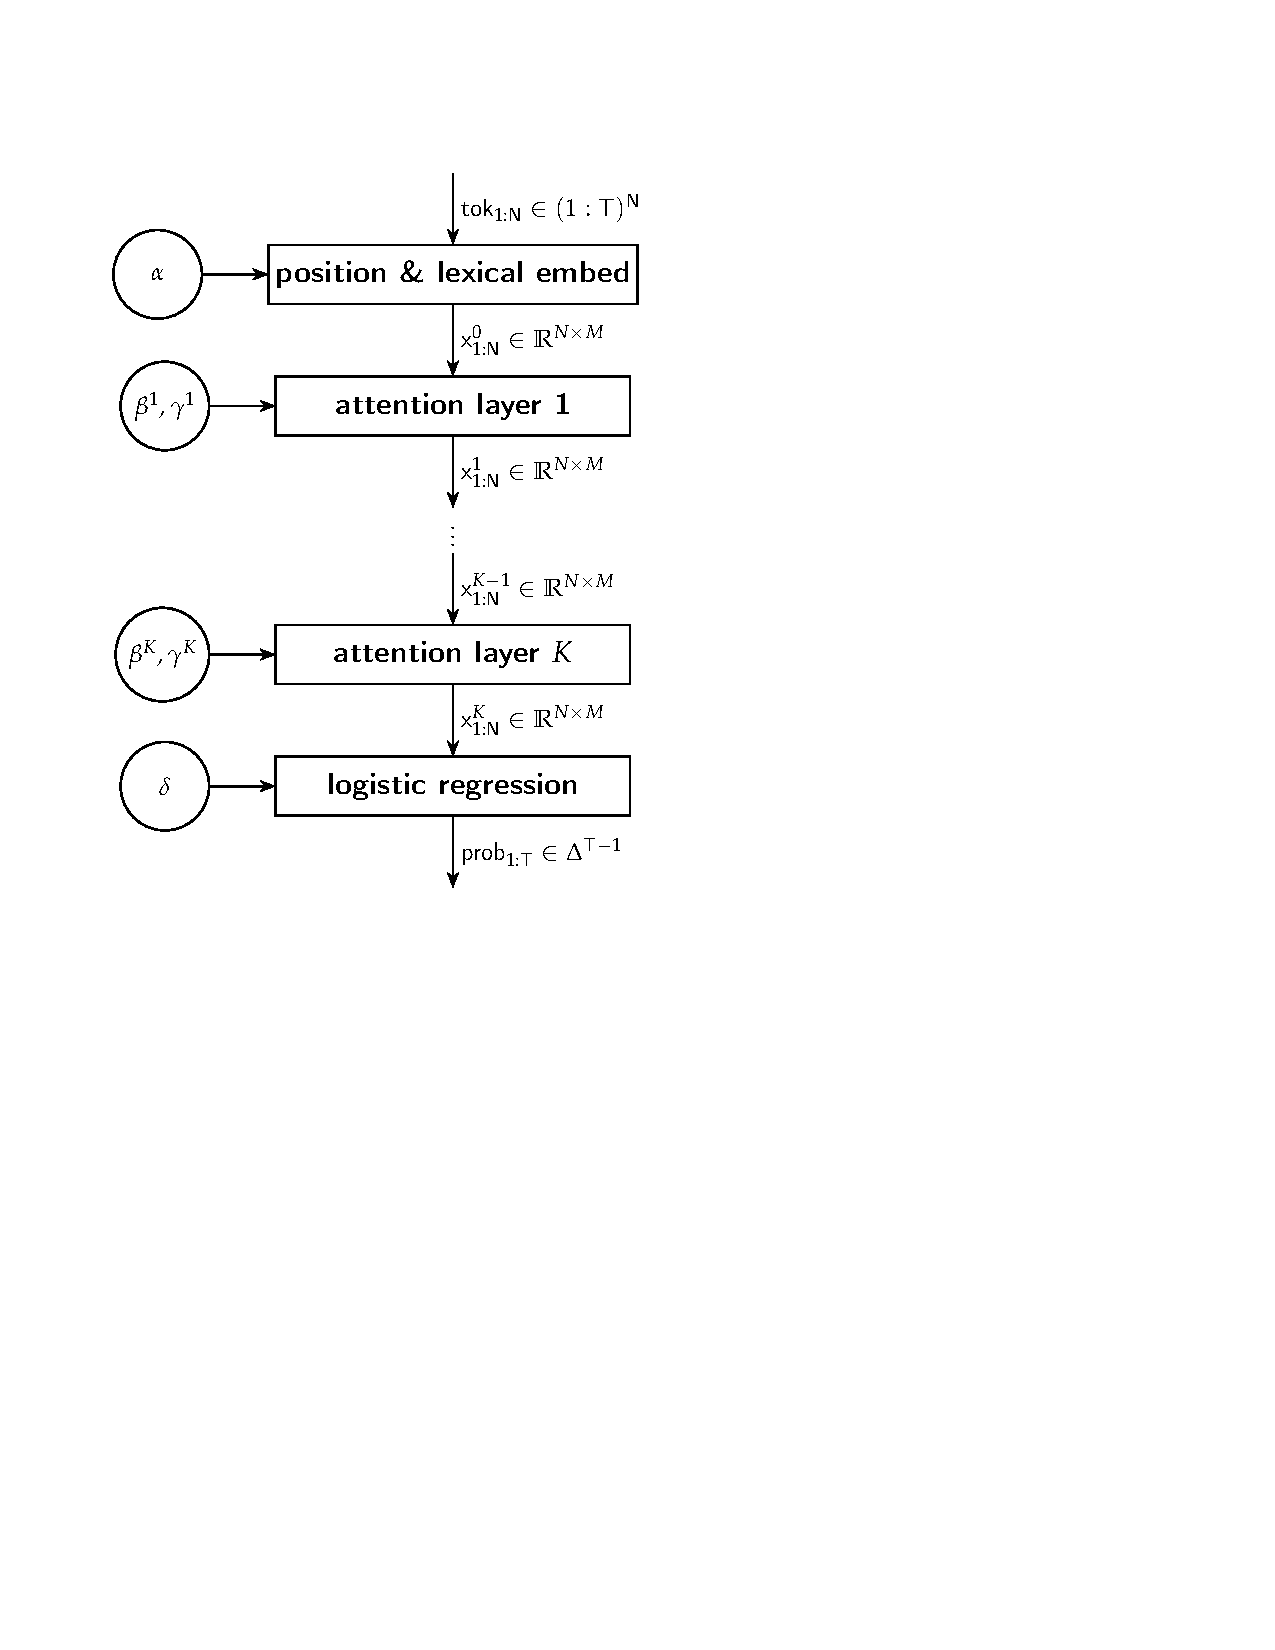
\includegraphics[height=\textheight]{img/transformer-diagram.pdf}

\sld{Attention architecture}
\begin{itemize}
\item attention then feedforward neural net
\item \myemph{ResNet architecture}: tees to add input
  \begin{subitemize}
  \item $\approx$ \myemph{hierarchical model} of differences
  \item non-centered parameterization
  \end{subitemize}
\item standard two-layer \myemph{neural nets}
  \subit{\myemph{shared params} for each value}
\item \myemph{standardized} for numerics
\end{itemize}
\vspace*{-2in}
\hfill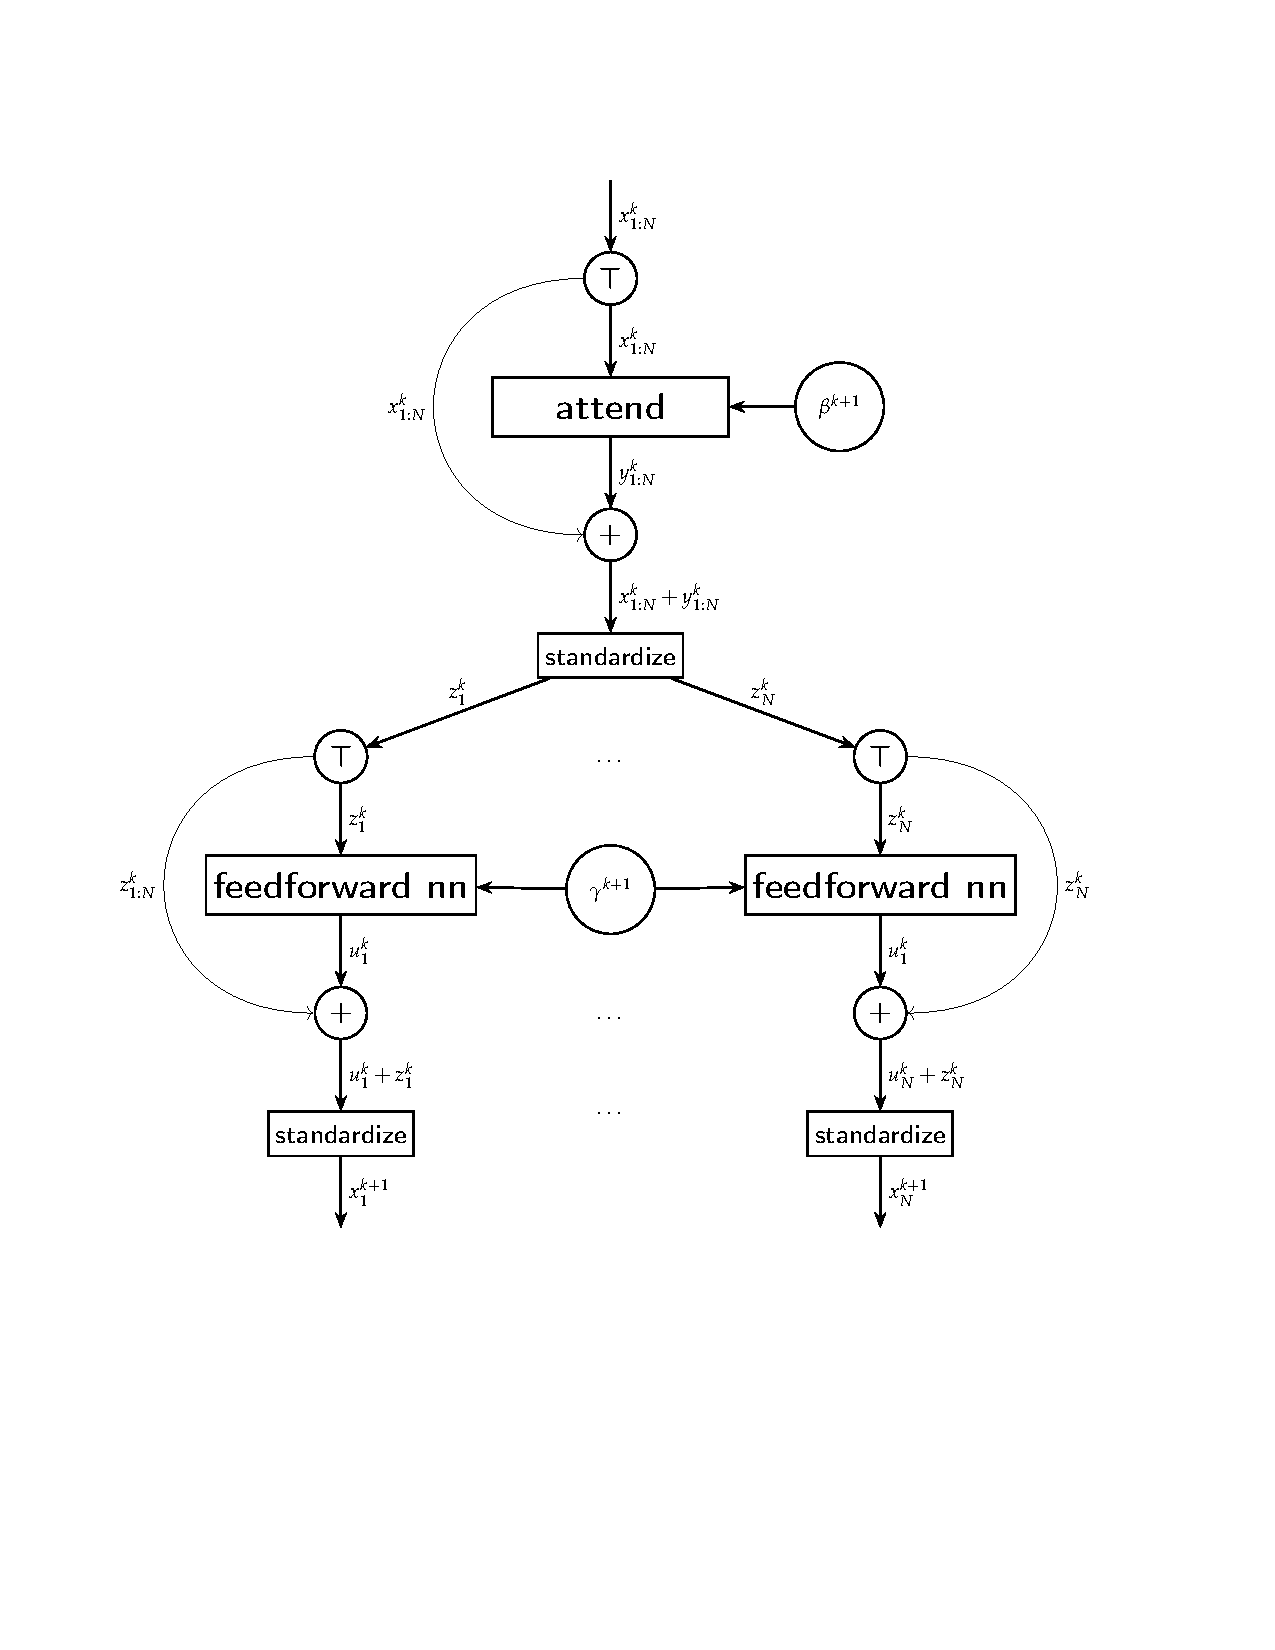
\includegraphics[height=\textheight]{img/attention-diagram.pdf}

\sld{Pseudocode: GPT in 40 lines}

\renewcommand{\baselinestretch}{1.1}
\footnotesize
\begin{verbatim}
    SIZES
    ------------------------------------
    T:  number of distinct tokens
    N:  size of context (history)

    V:  size of token embedding vectors
    A:  number of attention layers
    K:  size of keys and queries
    L:  width of neural network
\end{verbatim}

\clearpage
\footnotesize 
\begin{verbatim}
     DECODE(tok:  int<low=1,up=T>[N],    alpha:  matrix(T, V),
            betas: { query:matrix(K, V),
                     key:matrix(K, V),
                     value: matrix(V, V) }[A]
            gammas:  nn(V, L)[A],
            delta:   {1: vector[T],
                      2: matrix(T, N * V)}): simplex[T]
     ----------------------------------------------------------
     for n in 1:N:
         xs[0, n] = LEX(tok[n], alpha) + POS(n)
     for a in 1:A:
         xs[a] = ATTEND(xs[a - 1], betas[a], gammas[a])
         for n in 1:N:
             xs[a, n] = FEED_FORWARD(xs[a, n], gammas[a])
     y = STANDARDIZE(delta.1 + delta.2 * xs[A].flatten())
     return SOFTMAX(y)
\end{verbatim}
\normalsize

\clearpage
\footnotesize
\begin{verbatim}
      LEX(t:      int<low=1,up=T>,
          alpha:  vector(V)[T]):  vector(V)  
      ----------------------------------------------------------
      return alpha[t]


      POS(n:  int<low=1,up=N>):  vector(V)
      ----------------------------------------------------------
      for i in 1:V / 2:
          r = n / N**(2 * i / V)      // pos / max_pos^(0..2]
          u[2 * i] = sin(r)
          u[2 * i + 1] = cos(r)
      return u
\end{verbatim}

\clearpage
\footnotesize
\begin{verbatim}
      ATTEND(x:      vector(V)[N],
             beta:   { query: matrix(K, V), key: matrix(K, V),
                       value: matrix(V, V)},
             gamma:  nn(V, L)):  vector(V)[N]
      -----------------------------------------------------------
      for n in 1:N:
          q[n] = beta.query * x[n]
          k[n] = beta.key * x[n]
          v[n] = beta.value * x[n]
      for n in 1:N:
          lp[1:n-1] = [q[n]' * k[1], ..., q[n]' * k[n-1]] / sqrt(V)
          lp[n:N] = -inf                                 
          p = SOFTMAX(lp)                                
          u[n] = SUM(n in 1:N) p[n] * v[n]               
          y[n] = STANDARDIZE(u[n] + x[n])                
      return y
\end{verbatim}

\clearpage
\begin{verbatim}
     FEED_FORWARD(x:     real[R], 
                  alpha: { 1: real[S], 2: real[S, R], 
                           3: real[R], 4: real[R, S]):  real[R]
     ----------------------------------------------------------
     u = alpha.1 + alpha.2 * x
     v = GELU(u)              
     y = alpha.3 + alpha.4 * v
     return STANDARDIZE(x + y)

     GELU(v:  real[R]):  real[R]
         return [v_i * Phi(v_i) for v_i in v]

     STANDARDIZE(v:  real[R]):  real[R]
         return (v - mean(v)) / std_dev(v)

     SOFTMAX(real[R] v):  simplex(R)
         return exp(v) / sum(exp(v))
\end{verbatim}
\normalsize
\renewcommand{\baselinestretch}{1}

\sld{Multi-head attention}
\begin{itemize}
\item What we have presented is \myemph{single-head attention}
\item In practice, GPT uses \myemph{multi-head attention}
  \begin{subitemize}
    \item $J$ parallel attention ``heads''
    \item keys, values, queries for each head \myemph{projected from
        previous layer value}
    \item \myemph{value projected} for each head down to size to $V / J$
    \item \myemph{concatenate} output of each head to produce size $V$ value
    \end{subitemize}
\item GPT-4 rumored to use parallel GPTs in an ensemble
\end{itemize}

\sld{GPT-3 sizes}
\begin{itemize}
\item 175 billion parameters 
\item 96 layers 
\item 12,288 total value width 
\item 96 parallel attention heads 
  \subit{128 value width per head}
\end{itemize}

\sld{From LLM to Chatbot}
\begin{itemize}
\item \myemph{LLM goal}: predict \myemph{next token on web} page
\item \myemph{Chatbot goal} is to train a model that is
  \begin{subitemize}
  \item \myemph{helpful}: help users solve task
  \item \myemph{honest}: shouldn't fabricate or mislead user
  \item \myemph{harmless}: shouldn't cause physical, psychological,
    social, or environmental harm
  \end{subitemize}
\item Strategy is to \myemph{align} an LLM to be a Chatbot with
  \myemph{fine tuning}
  \begin{subitemize}
  \item LLM acts as an \myemph{informative prior}
  \item In ML terms, LLM provides \myemph{inductive bias}
  \end{subitemize}
\end{itemize}

\sld{Reinforcement learning with human feedback \\ \null\hspace*{1em}(RLHF)}
\begin{enumerate}
\item Supervised fine tuning
  \begin{subitemize}
  \item human raters \myemph{provide desired output} for sampled prompts
  \item \myemph{fine-tune} LLM with \myemph{supervised learning}
  \end{subitemize}
\item Reward model training
  \begin{subitemize}
  \item human raters \myemph{rank multiple outputs} for sample prompts
  \item train a \myemph{reward model}
  \end{subitemize}
\item Reinforcement learning
  \begin{subitemize}
  \item \myemph{policy ranks outputs} for sample prompts
  \item fine-tune LLM with \myemph{proximal policy optimization} (PPO)
  \end{subitemize}
\end{enumerate}

\sld{Some caveats (OpenAI 2022)}
\begin{itemize}
\item 
{\LARGE ``\null}This procedure aligns the behavior of GPT-3 to the \myemph{stated preferences of a
specific group} of people (mostly our labelers and researchers), rather
than to any \myemph{broader notion of ``human values''}.
\subit{cf. \myemph{Cultural consensus theory} provides mixture model of
  ``values''}
\vfill
\item {\LARGE ``\null}During RLHF fine-turning, we observe \myemph{performance
    regressions} compared to GPT-3 on certain public NLP
  datasets.
  \begin{subitemize}
  \item i.e., performance degrades relative to unaligned model
  \item partially mitigated by \myemph{hierarchical modeling}
    alternating reinforcement and supervision
  \end{subitemize}
\end{itemize}

\sld{Loss vs.\ tokens, model size \hfill (OpenAI)}
\begin{itemize}
\item Accuracy is \myemph{bounded by parameter size} (right)
\item Accuracy is \myemph{bounded by data size} (left)
  \\[8pt]
  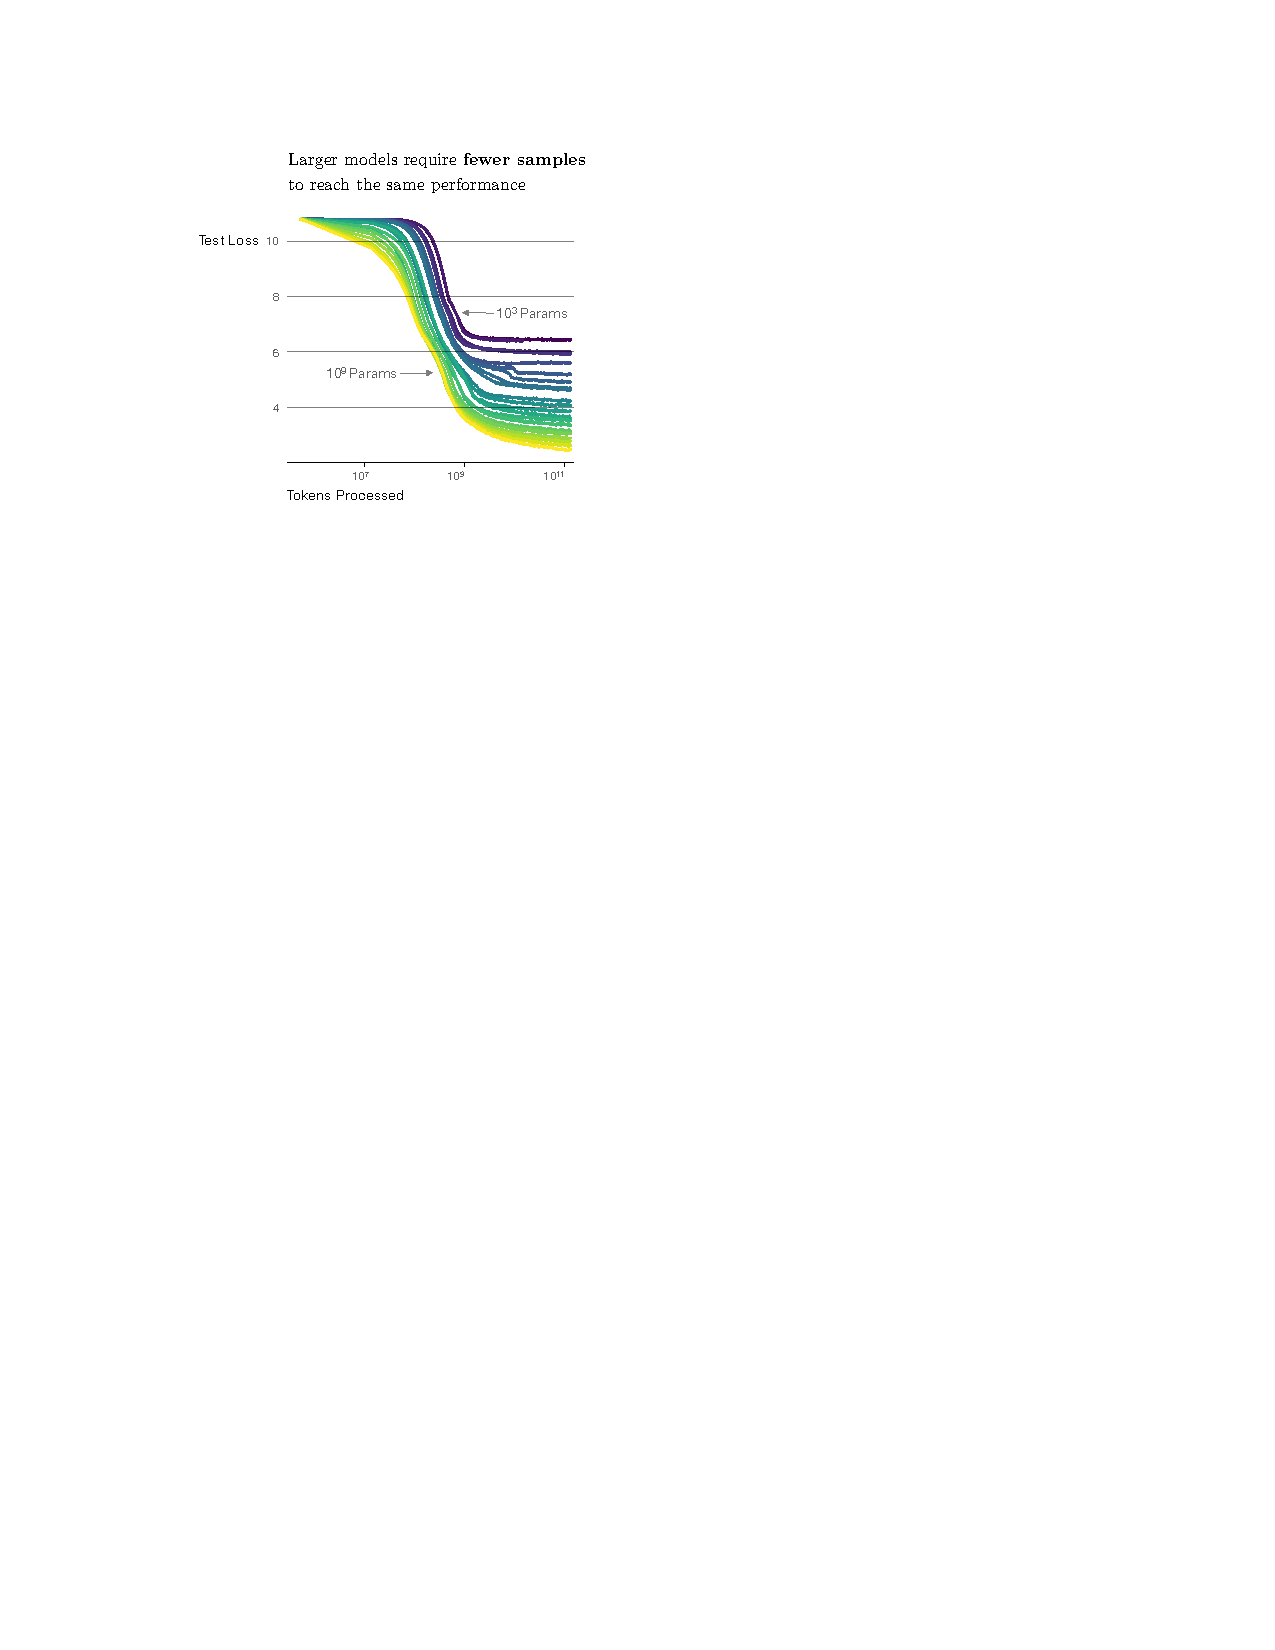
\includegraphics[height=0.6\textheight]{img/accuracy-vs-tokens-size.pdf}
  \quad
  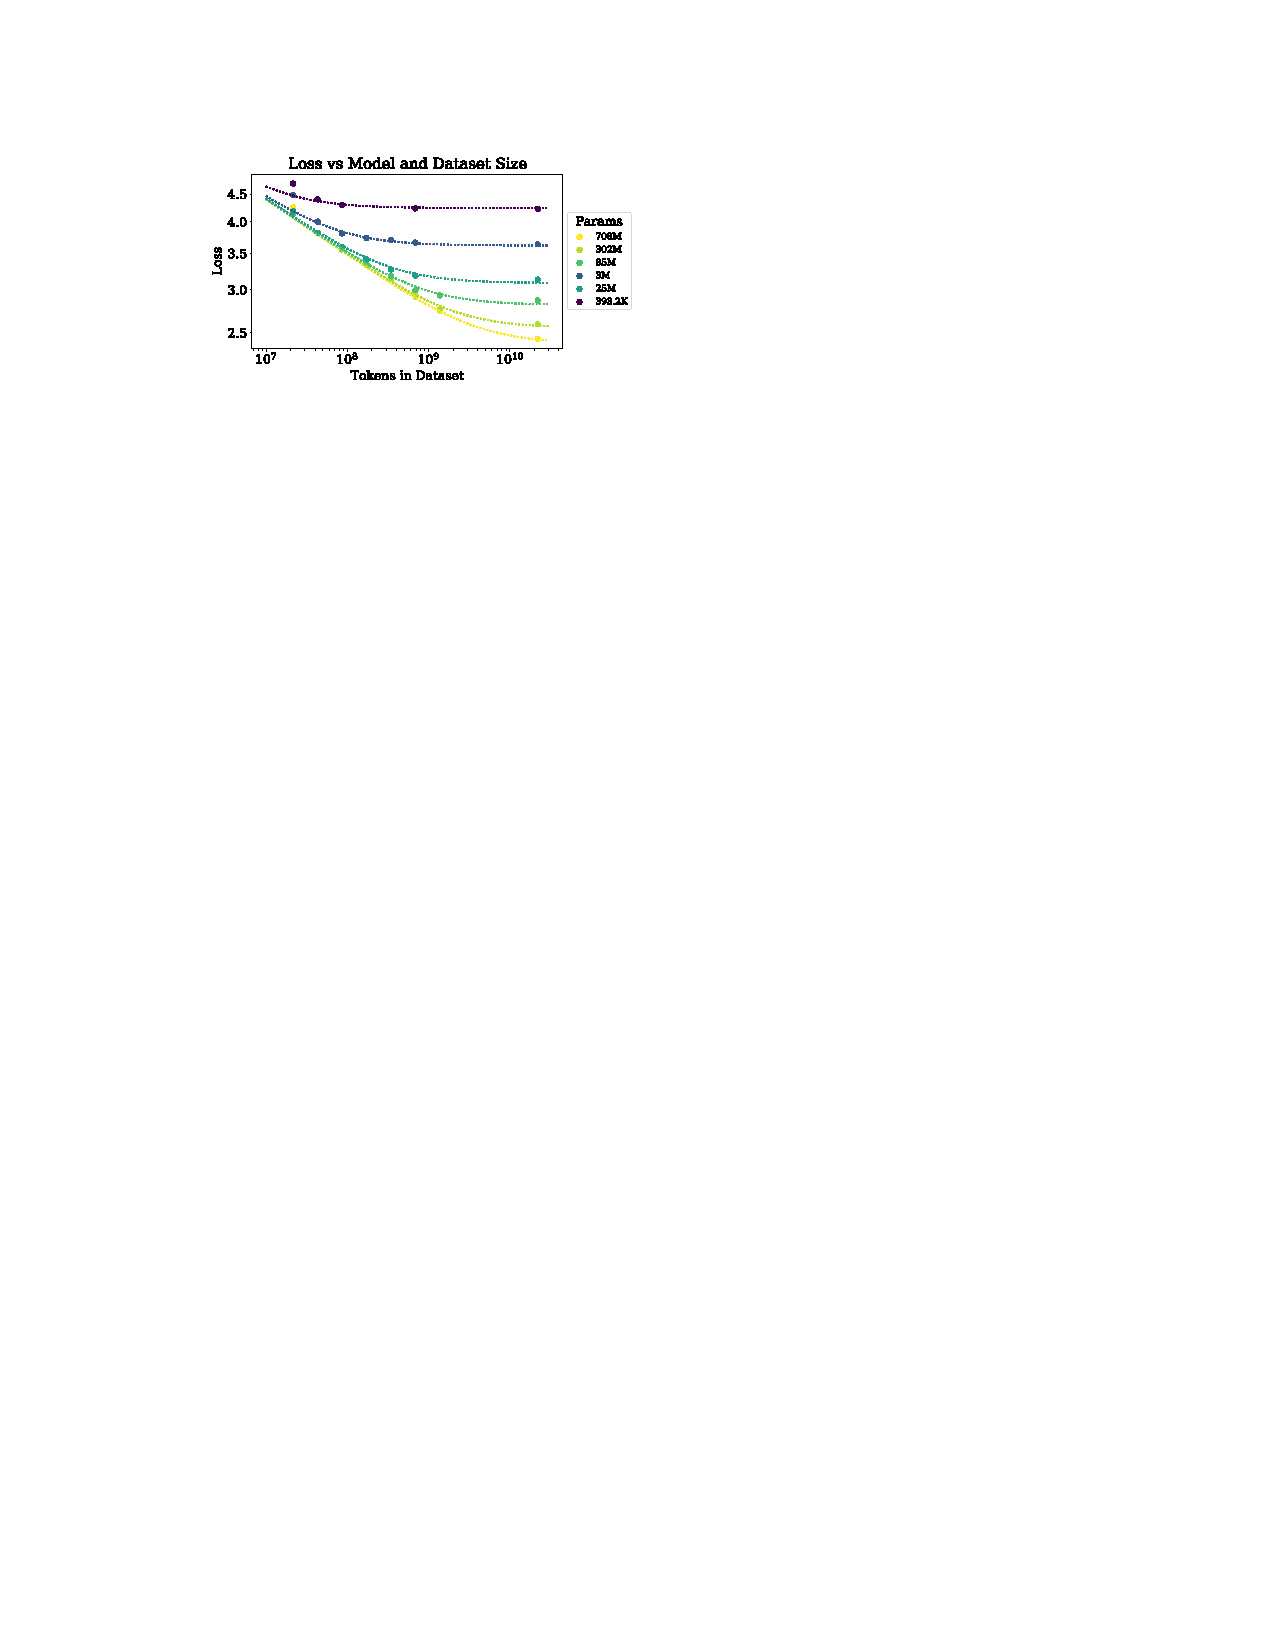
\includegraphics[height=0.6\textheight]{img/loss-vs-model-dataset-size.pdf}
\end{itemize}

\sld{Scaling models \hfill (DeepMind)}
\begin{itemize}
\item Accuracy \myemph{determined by flops}
  \begin{subitemize}
  \item for given \myemph{flops}, there is an \myemph{optimal choice} of
    \myemph{training tokens} and \myemph{model size}
  \item fits held out predictions \myemph{very well}
  \end{subitemize}
  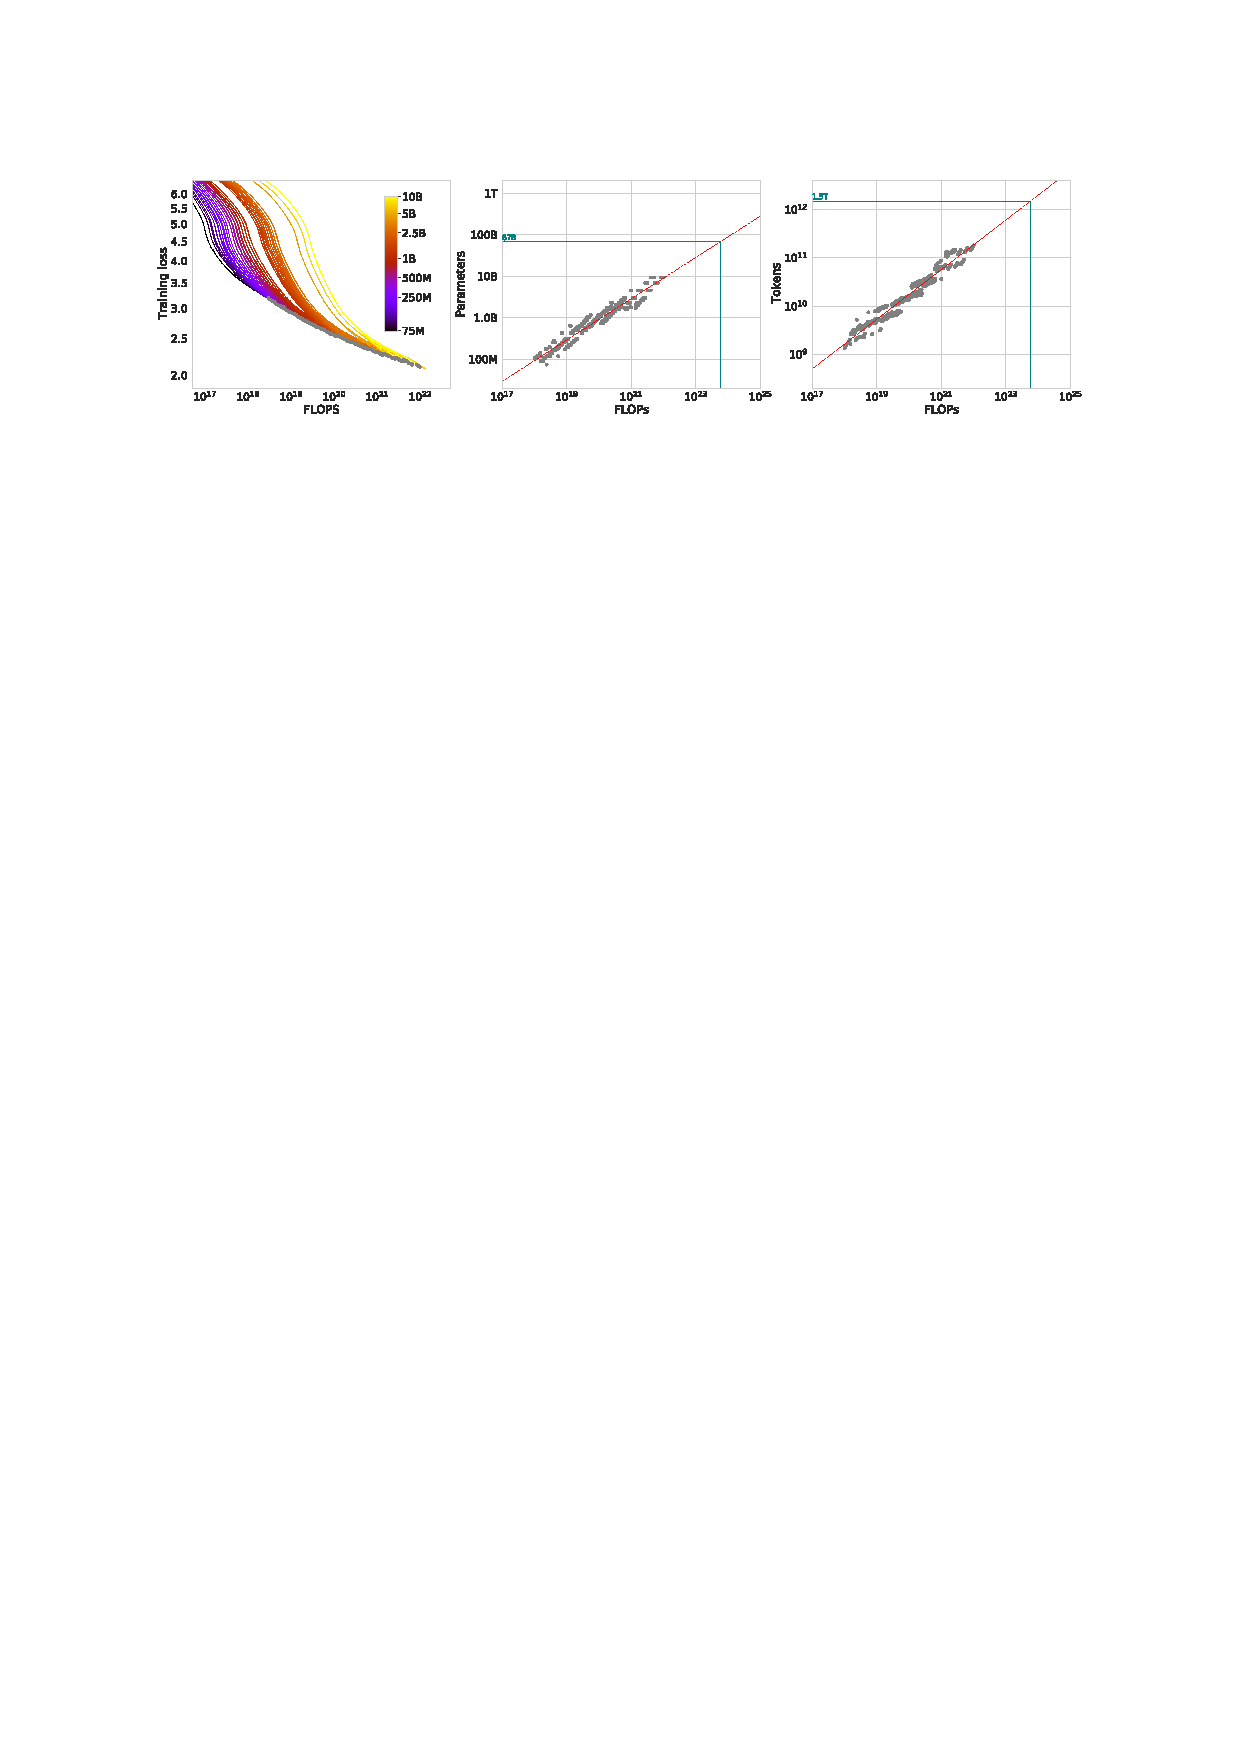
\includegraphics[width=\textwidth]{img/flops-chinchilla.pdf}
  \vspace*{-12pt}
  \subit{(l) loss by model size, (c) optimal parameters, (r) optimal train tokens}
\end{itemize}

\sld{OpenAI's GPT-4: Unpublished}
\begin{itemize}
\item \myemph{Training set} unpublished (estimated $\approx$5 trillion)
\item \myemph{Parameter set} unpublished (estimated $\approx$2
  trillion)
\item \myemph{Context history size}: 8K or 32K tokens
\item \myemph{Cluster cost} training: $\approx$US\$500 million
  (incl.\ 10K+ US\$15K GPUs)
\item \myemph{Marginal cost} training: $\approx$US\$10s of
  millions (hardware, power, staff)
  \vfill
\item \myemph{Open AI} is now \myemph{ClosedAI}: {\small ``Given both
the competitive landscape and the safety implications of large-scale models like GPT-4, \myemph{this report
contains no further details} about the architecture (including model size), hardware, training compute,
dataset construction, training method, or similar.''}
\end{itemize}

\sld{The cat's out of the bag}
\begin{itemize}
\item Transformer LLM architecture published by \myemph{Google} (2017)
\item Alignment to ChatBots published by \myemph{OpenAI} (2022)
\begin{subitemize}
\item Meta (nee Facebook): \myemph{LLaMA}
  \vspace*{3pt}
  \begin{subitemize}
    \item \myemph{Open source} for research (since leaked)
    \item Stanford CS: \myemph{Alpaca} fine-tuned
    \item Runs 2 tokens/second on iMac with 4-bit floating point
    \end{subitemize}
  \item Google: \myemph{Bard}
  \item Google and OpenAI: \myemph{Copilot} (code/programming API integration)
\item Anthropic: \myemph{Claude} (100K token context) (branded as \myemph{Poe} for writing) 
\item Many smaller, less widely used alternatives
\end{subitemize}
\end{itemize}


\sld{LLM References}
\begin{enumerate}
\item \textit{The transformer paper}:
  \\[4pt]
  Vaswani et al. (Google). 2017. \hfill (82K~citations) 
  \\
  \myemph{Attention is all  you need}. \textit{NeurIPS}.
\item \textit{LLMs are highly generalizable}:
  \\[4pt]
  Brown et al. (OpenAI). 2020.  \hfill (12K~citations)  
  \\ \myemph{Language models are few-shot
    learners}. \textit{NeurIPS}.
\item \textit{Going from GPT to ChatGPT}:
  \\[4pt]
  Ouyang et al. (OpenAI). 2022.  \hfill (1.5K~citations)
  \\
  \myemph{Training language models to follow instructions}.
  \textit{NeurIPS}.
\clearpage
\item \textit{Original OpenAI paper on scaling}:
  \\[4pt]
  Kaplan et al. 2020. \hfill (0.6K~citations)
  \\
  \myemph{Scaling laws for neural language models}. \textit{arXiv}
\item \textit{Chinchilla paper on scaling laws for transformers}:
  \\[4pt]
  Hoffmann et al. (DeepMind) 2022. \hfill (0.1K citations)
  \\
  \myemph{Training compute-optimal large language models}. \textit{arXiv}
\item \textit{What can GPT-4 do?}
  \\[4pt]
  Bubeck et al. (Microsoft). 2023.  \hfill (0.4K~citations)
  \\ \myemph{Sparks of artificial general intelligence}. \textit{arXiv}.
\clearpage
\item \textit{Another pseudocode I found after I did mine}:
  \\[4pt]
  Phuong \& Hutter (DeepMind). 2022.  \hfill (0.02K~citations) 
  \\ \myemph{Formal algorithms for 
    transformers}. \textit{arXiv}. 
\item \textit{Reproducible PyTorch case study with Colab notebook fitting Shakespeare}:
  \\[4pt]
  Andrej Karpathy (now at OpenAI). 2023. \hfill (2.8M views)
  \\ \myemph{Let's build GPT: from scratch, in code, spelled out}. YouTube!
\end{enumerate}

\end{document}
